%!TEX root = ../../dissertation.tex

\section{Processing Techniques} % (fold)
\label{sec:processing_techniques}

Within the following section, a number of techniques that can be applied to improve performance of the processing and visualization of large amounts of geometry will be presented. First the \gls{LOD} in Section~\ref{sub:level_of_detail} which manages the detail that each object is generated with, and after that the \gls{OC} that manages which objects are generated.



\subsection{Level Of Detail -- JUST A COPY} % (fold)
\label{sub:level_of_detail}

Level of Detail is a technique that is used to improve the performance of the graphic pipeline. This is done by managing the complexity of the objects representation relative to some indicator.
Within this indicators, the most common one is the distance of each object to the viewer. If an object is far from the viewer a decrease on the detail will not be noticed and will save computation time. Other indicators can be the importance that is assigned for each object, relative speed or partial occlusion.

This concept is easy to understand and implement if we look at the example in the Figure~\ref{fig:LOD2}. In this figure there are five cylinders that have different detail according to the distance to the camera. In this case only the number of sides of the cylinder changes.

%\begin{figure}[htbp]
%	\centering
%	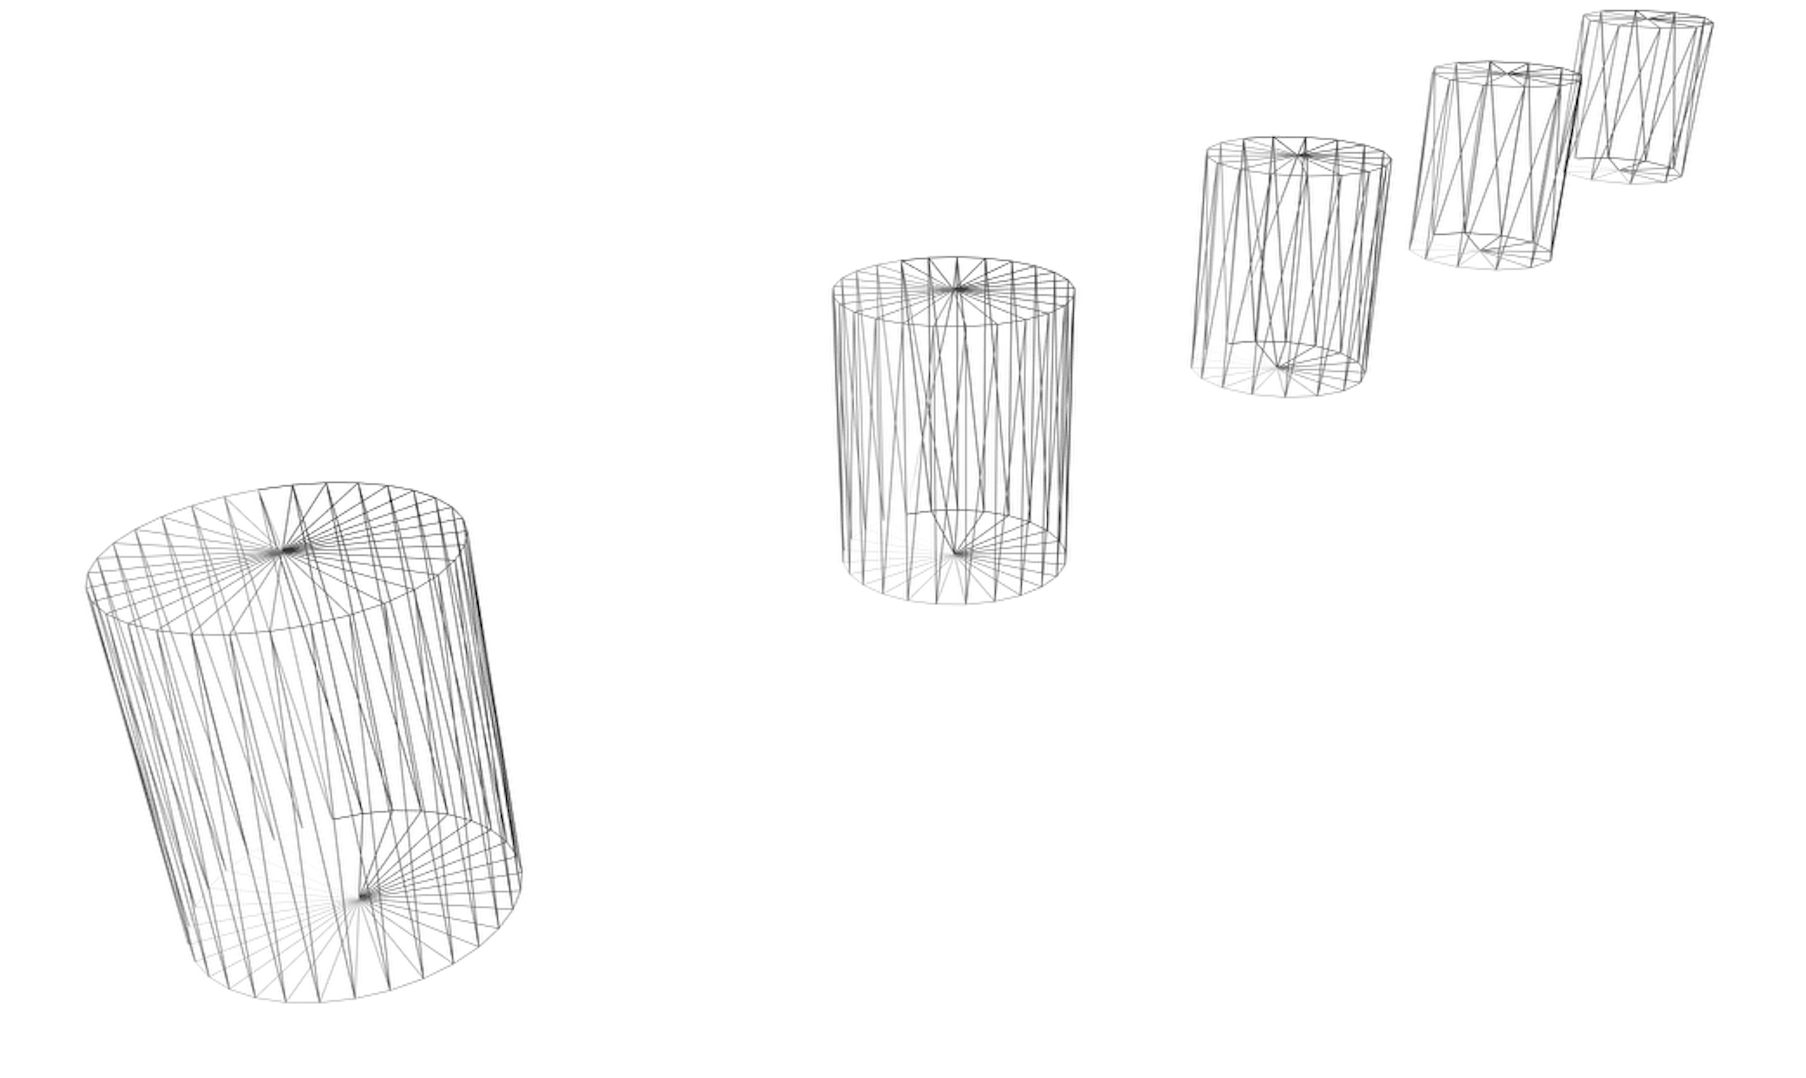
\includegraphics[width=0.95\textwidth]{imges/OpenGL/LOD3.png}
%	\caption{LOD example}
%	\label{fig:LOD2}
%\end{figure}


% subsection level_of_detail (end)

\subsection{Occlusion Culling} % (fold)
\label{sub:occlusion_culling}

Occlusion Culling is another technique that is used to improve performance. It involves determining which parts of the model are visible or not at any given moment, and with that information remove the not visible parts of the pipeline.

This technique can be implemented in different phases of the system. This can be implemented by the programmer when generating the models, only generating the parts that are visible according the the camera. But it is not easy to implement and therefore is not a good neither popular solution.

On the other end of the pipeline, it is usually done automatically by the GPU and applied to occluded faces behind other objects or out of the viewing frustum. This solution is not great because all the model is generated and, is only after that occlusion culling is applied which doesn't translate in grate performance gains.

If this concept is applied before the generation of the objects, and prevents the inclusion of large amounts of geometry through the pipeline, we can make a large improvement on performance. Figure~\ref{fig:viewingRange} is a good example. Here only the buildings that are visible from the current point are generated. This test is done prior to the generation of each object and is not hard coded within the model description.

% subsection occlusion_culling (end)

% section processing_techniques (end)

		